\documentclass{article}

\usepackage{../mathclub}

\title{Graphy Things} 
\author{}
\date{April 25, 2022}

\begin{document}

\section{Introduction}
Welcome to Week 5 of Math Club! Last quarter, we took a first stab at Graph Theory. Today, we will repeat this criminal offense and expand on a certain historical Graph Theory problem. That is, we will be taking a closer look at the Three Utilities Problem, along with its connections to topology. Without a further ado, a doodoo.

\section{Basic Definitions} 
\begin{definition}
A finite simple graph is a pair $G = (V, E)$ of sets $V = \{v_{1}, v_{2}, \ldots, v_{n}\}$ and $E = \{e_{1}, e_{2}, \ldots, e_{m}\}$ where elements in $V$ are called vertices and elements of $E$ are called edges where each is a $2$-element subset of $V$. 
\end{definition}

\begin{definition}
A walk in $G = (V, E)$ is a sequence $(v_{1}, e_{1}, v_{2}, \ldots, e_{k}, v_{k + 1})$ where each $e_{i} = v_{i}v_{i + 1}$. The length of a walk is the number of edges traversed. A path is a walk with no vertices repeated. A cycle is a walk with no vertices repeated except the endpoints.
\end{definition}

\begin{definition}
A graph $G = (V, E)$ is connected if for every pair $u, v \in V$, there's a $(u, v)$-walk. 
\end{definition}

\begin{definition}
A circuit is a closed walk where any edge is used at most once. Eulerian circuit is a circuit that uses every edge exactly once. 
\end{definition}

\begin{definition}
The degree of a vertex $v$ in $G$, denoted by $\deg(v)$, is the number of edges incident to $v$. 
\end{definition}

\begin{definition}
The chromatic number $\chi(G)$ is the smallest number of colors needed so that each no adjacent vertices are the same color.
\end{definition}

\begin{definition}
The complement $\overline{G}$ of $G$ is the graph where we draw every edges between every pair of vertices in $G$ that are not adjacent.
\end{definition}

\begin{definition}
The graph $G = (V, E)$ is planar if it can be embedded in $\mathbb{R}^{2}$ such that no edges cross. 
\end{definition}

\section{Useful Theorems}

\begin{theorem}(Kuratowski)
A finite graph $G$ is planar if and only if it does not contain a subgraph that is homeomorphic to $K_5$ or $K_{3,3}$.
\end{theorem}

\begin{theorem}(Euler's formula)
If $G$ is a planar-connected graph with $v$ vertices, $e$ edges, and $f$ faces, then $v - e + f = 2$. 
\end{theorem}

\section{Three Utilities Problem}
\begin{center} 
    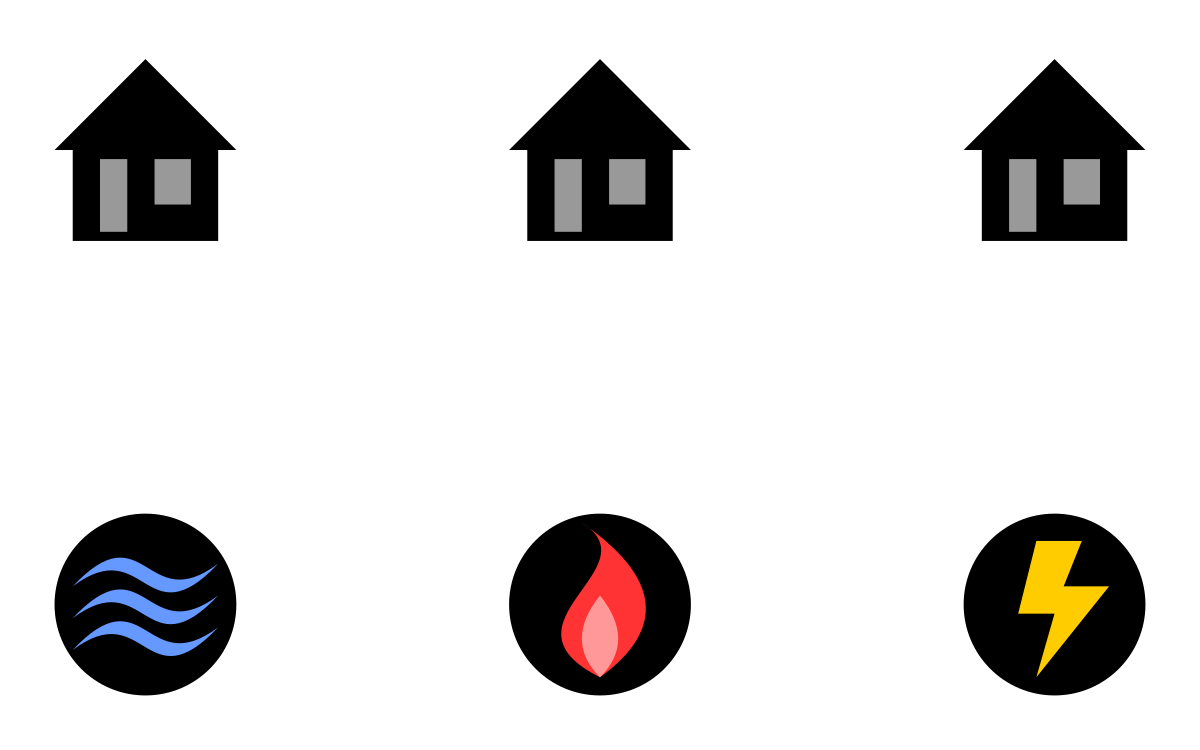
\includegraphics[scale=0.3]{Pics/utilities.png}

\end{center}

\begin{exercise}
It is fairly well-known that the Three Utilities Problem is impossible, so go ahead and try to convince yourself you absolute fool.
\end{exercise} 
\begin{exercise}
Prove that the Three Utilities Problem is actually impossible. In other words, prove that $K_{3,3}$ is non-planar without Kuratowski's Theorem. \emph{Hint: Look above!}.
\end{exercise}
\begin{exercise} 
Now that we've determined that the Three Utilities Problem is impossible on $\mathbb{R}^2$, we turn our attention to sweeter topological spaces, namely donuts! 
(At this point, you should bother Neel about where the donuts are.) Is the Three Utilities Problem possible on a Torus?
\begin{center} 
    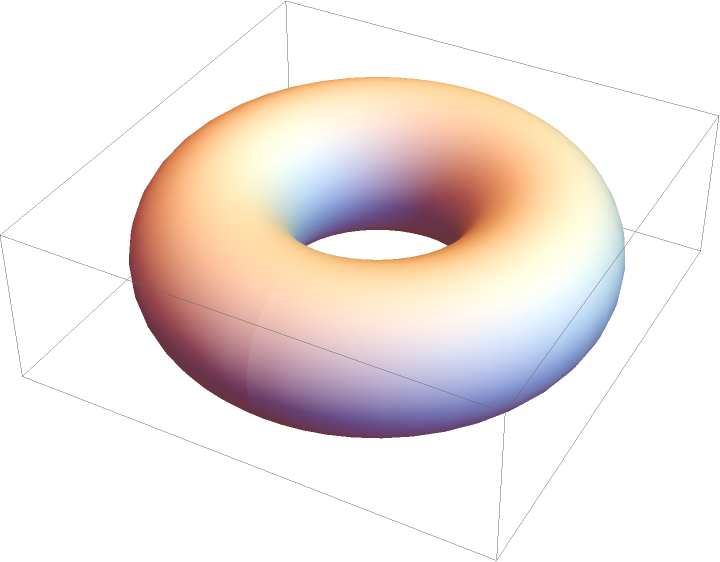
\includegraphics[scale=0.3]{Pics/yum.png}
\end{center}
\end{exercise}
\begin{exercise} 
Justify why the Three Utilities Problem can be solved on the surface of a Torus. Is there something \emph{fundamentally} different about
$\mathbb{R}^2$ and the Torus? Try to play around with Euler's formula! Does the same formula hold?
\end{exercise}
\section{Euler Characteristic and Topological Invariants}
    Spoilers: there is something in fact different about the Real Plane $\mathbb{R}^2$, and the Torus. In mathematical terms, the two topological spaces 
    are not homeomorphic. In the motivating example above, we've successfully determined the two spaces have differing \emph{Euler Characteristics}. The 
    Euler Characteristic is one of many examples of a Topological Invariant, a property that stays the same under homeomorphism. Topological Invariants are tools 
    that help us determine whether two topological spaces are ``the same." 
    \begin{exercise} 
        Can the Three Utilities Problem be solved on these topological spaces? Furthermore, which of the following spaces are not homeomorphic?
        \begin{align*} 
            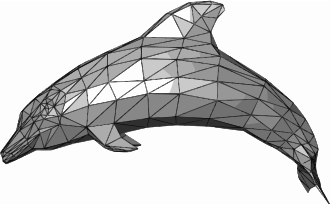
\includegraphics[scale=0.25]{Pics/dolp.png} ~~~~~ 
            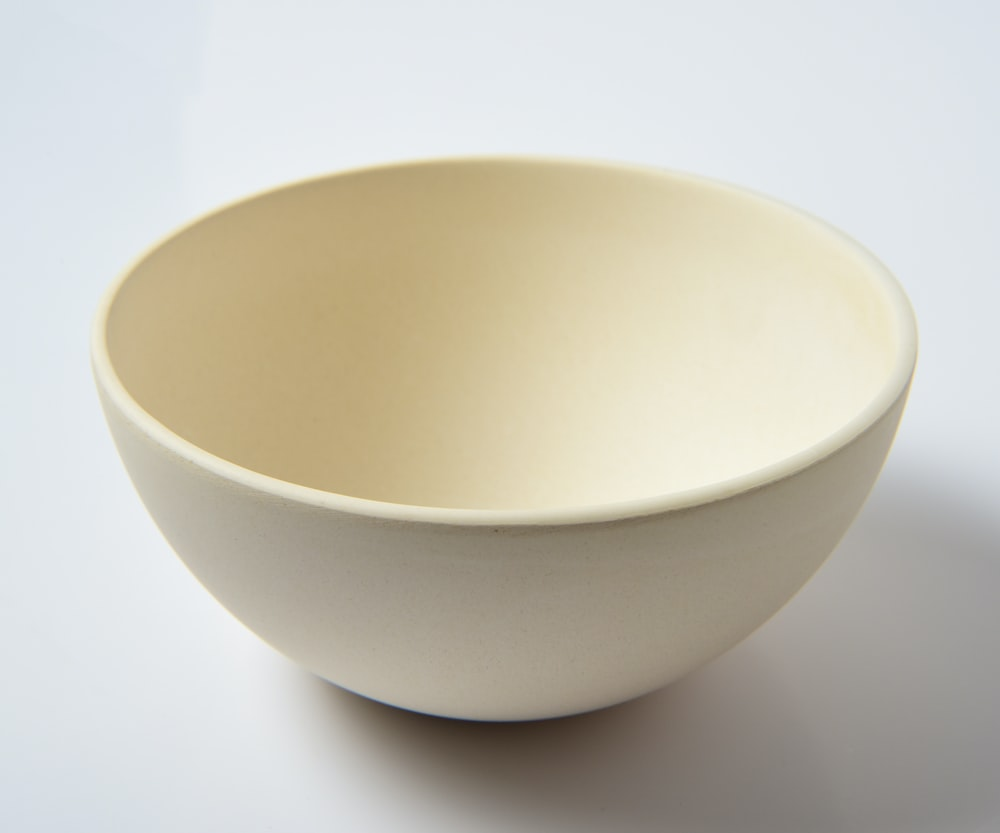
\includegraphics[scale=0.08]{Pics/bowl.jpg} ~~~~~~ 
            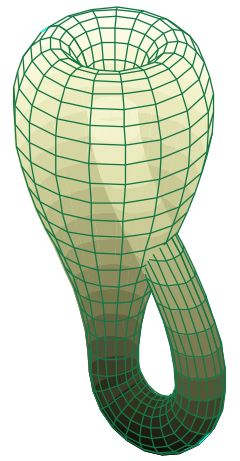
\includegraphics[scale=0.15]{Pics/ddw.png} ~~~~~ 
            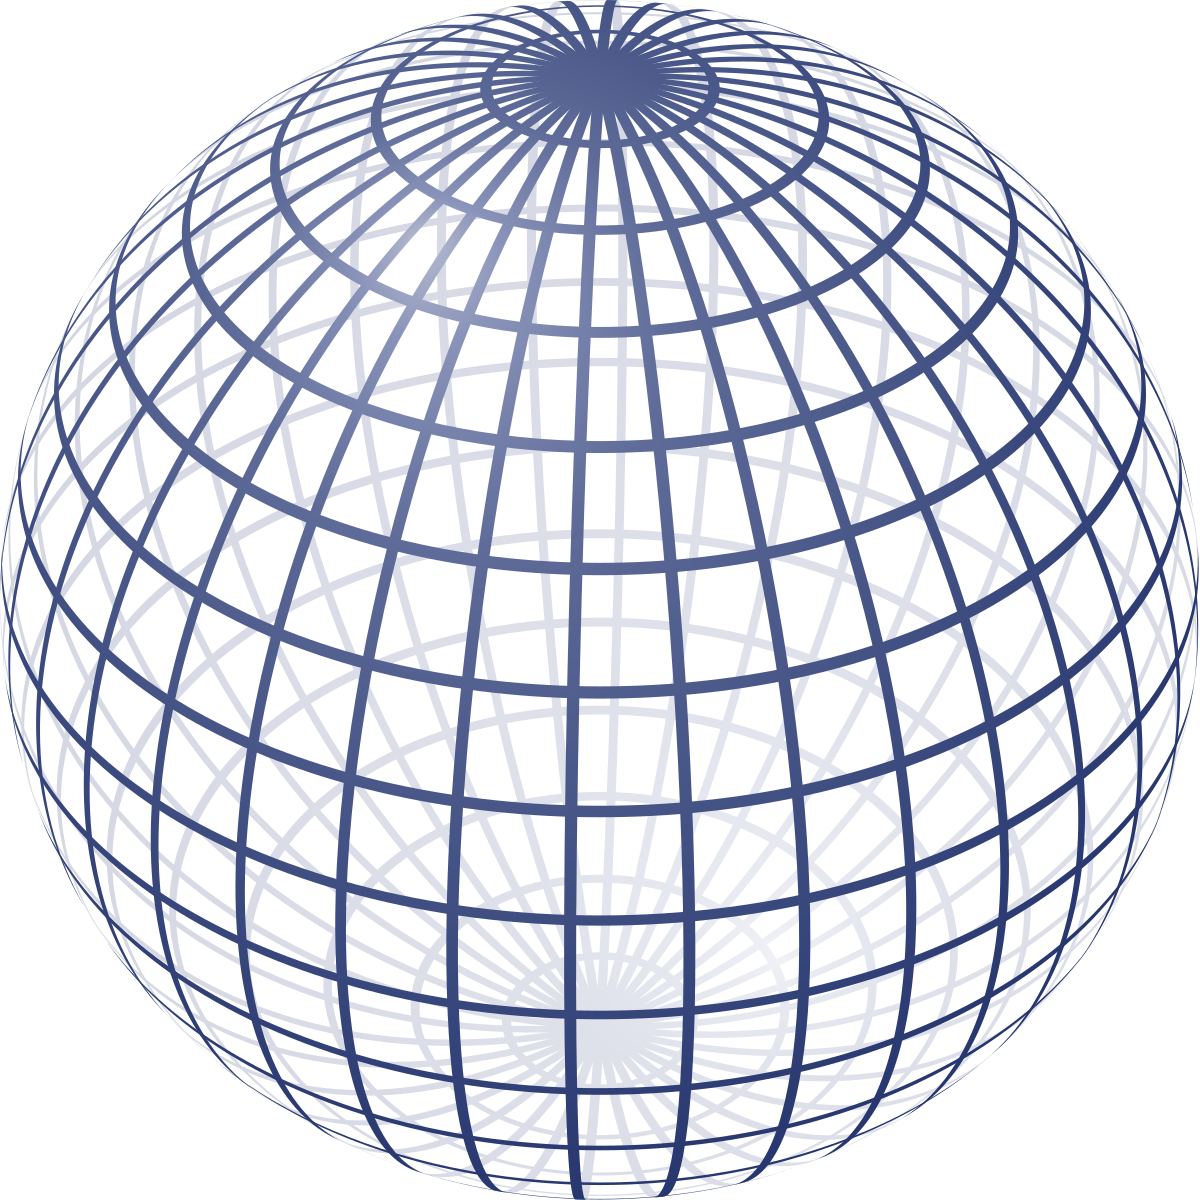
\includegraphics[scale=0.06]{Pics/dog.png} ~~~~ 
            
\includegraphics[scale=0.35]{Pics/s-l300.jpg}
        \end{align*}
    \end{exercise}
    As you may have noticed, though the sphere and the (infinite) sheet of paper may have the same Euler Characteristic, the spaces are very much so not homeomorphic!
    That is, $S_2$ is compact but $\mathbb{R}^2$ is very not compact. In other words, two homeomorphic spaces must have the same Euler Characteristic, but the converse isn't true! 
\section{Further Readings}
    If you're still curious after this really brief introduction to the Euler Characteristic, please consider checking out ``Algebraic Topology" by Allen Hatcher! 
    There are tons of more sophisticated Topological Invariants, and I'm sure you'll find it exhilarating! (interesting?, amusing?, tolerable?, not despicable?)

\end{document}